\RequirePackage[T1]{fontenc}
\documentclass[conference]{IEEEtran}
\usepackage{cite}
\usepackage{graphicx}
\usepackage{booktabs}
\usepackage{siunitx}
\usepackage{url}
\DeclareSIUnit{\ppm}{ppm}
\DeclareSIPrefix{\micro}{\ensuremath{\mu}}{-6}
\graphicspath{{figures/}}

\begin{document}
\title{Cooperative Aerial Survey and Ground Confirmation of Industrial Hazards}
\author{\IEEEauthorblockN{Tom\'as Oliveira (1261742) and Hugo Amado (1261726)}
\IEEEauthorblockA{Instituto Superior de Engenharia do Porto\\
Porto, Portugal\\
RSDIS, Group 22, 2026/27}}
\maketitle

\begin{abstract}
This project implements a cooperative inspection mission with one aerial robot and two ground robots in an industrial Gazebo scenario. The site's obstacle map is known in advance, while hazard locations must be discovered during the mission. The aerial robot follows survey lanes and uses camera signs and simulated gas and radiation readings to identify locations for ground inspection. A coordinator assigns each candidate to the nearest available ground robot, which navigates with Nav2 and collects fresh measurements. The decision-making nodes have no access to source positions, simulated field models or background values. The scenario contains six active sources: four gas leaks and two radiation sources. It includes a gas leak without a matching warning sign and a radiation sign without a source. In three completed trials, positive ground checks were associated with all six reference sources, and each ground robot completed three checks. The last ground check occurred between 280.3 and 294.1 simulated seconds after logging began. Mean position errors per run were 1.48 to 1.51 metres for aerial candidates and 1.67 to 1.71 metres for ground checks. These results apply to the tested static fields and idealised aerial localisation. A positive ground check confirms an elevated local reading; it does not establish the exact source position.
\end{abstract}
\begin{IEEEkeywords}
multi-robot cooperation, ROS 2, Gazebo, hazard inspection, aerial survey, mobile navigation
\end{IEEEkeywords}

\section{Introduction}
An industrial inspection robot must distinguish a location worth investigating from a hazard supported by measurements. An aerial view can reveal labelled containers and cover routes above obstacles. Ground robots can then approach selected locations and measure closer to the source. This division of work is the basis of the mission developed for the RSDIS final project.

The objective is to implement a reproducible multi-robot application with a Gazebo scenario, custom perception and control nodes, and information sharing between robots. Robot Operating System 2 (ROS 2) provides the communication and execution environment~\cite{ros2}. The team consists of one unmanned aerial vehicle (UAV) and two unmanned ground vehicles (UGVs). The UAV surveys the site and publishes candidates; the UGVs perform ground checks. Nav2 supplies ground navigation~\cite{nav2}, while the project implements the inspection policy, task allocation, sensor interfaces and result logging.

The mission assumes an industrial facility whose layout is available before inspection. Walls, buildings and fixed equipment are already mapped; the unknown information is where gas or radiation readings are elevated. This choice makes inspection the main task. The robots share detections, ground measurements and task state in a common map frame. Simultaneous localisation and mapping (SLAM), map merging and exploration of unknown geometry are outside the chosen scope.

\section{Problem and Proposed Solution}
\subsection{Industrial inspection problem}
The simulated 36 by 28 metre site contains walls, a building, containers, tanks, vehicles and smaller obstacles (Fig.~\ref{fig:scenario}). Six active sources are configured independently of these objects: four gas leaks and two radiation sources. Several barrels can stand beside the same source, so barrel count and source count differ. Warning signs stand near five sources. Gas 4 has a black-diamond lookalike barrel at its location but no matching gas warning sign. A radiation-labelled barrel elsewhere has no source. These cases test detection from measurements alone and rejection of an unsupported visual cue. The task is to identify hazardous areas, obtain ground measurements and record their locations.

\begin{figure}[t]
\centering
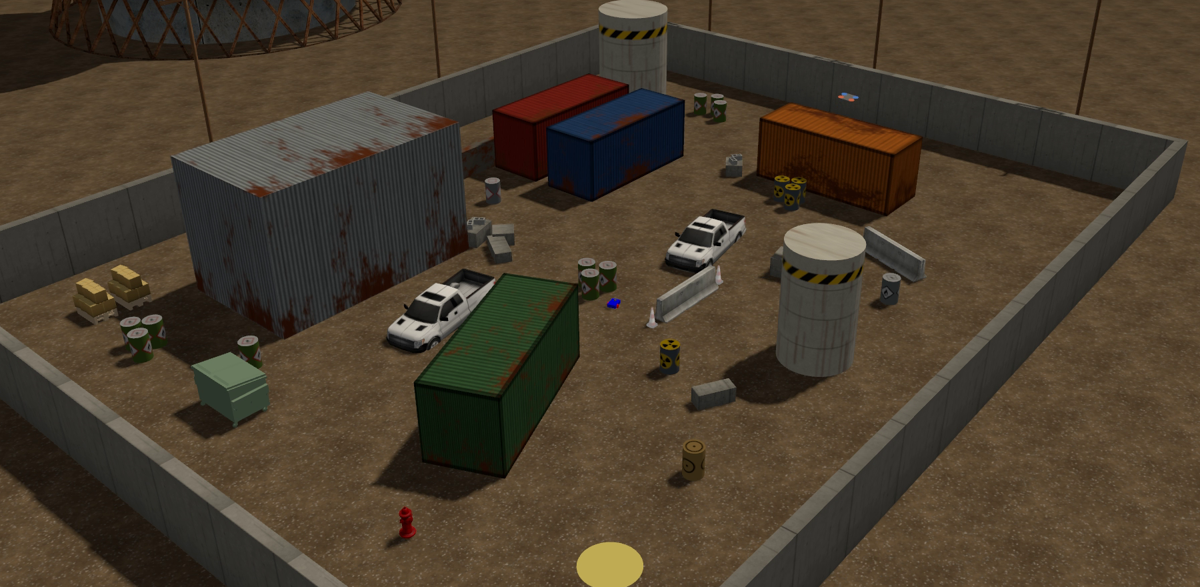
\includegraphics[width=\columnwidth]{scenario.png}
\caption{Gazebo view of the industrial site during a mission. The flight route passes above the obstacles; UGVs use the traversable ground corridors.}
\label{fig:scenario}
\end{figure}

A static occupancy map represents the known site layout at \SI{0.05}{\metre} resolution. In this simulation it is generated from the world's box and cylinder collision geometry before the mission. It represents the prior map that could be available from a facility plan or an earlier survey. Each UGV loads this map for localisation and navigation, and the coordinator uses it to select clear goals. The map contains obstacle geometry only. Signs, hazard candidates and ground readings are added from observations during the mission.

\subsection{Cooperative workflow}
After take-off, the UAV follows alternating parallel survey lanes. A warning sign requests an inspection at its estimated position. A sensor alarm without a pending sign starts a short local search. Both paths require measurements above the alarm threshold before a candidate is published. After each inspection, the UAV resumes its route. It returns home and lands after finishing the survey; ground checks continue independently. The UAV has no configured source count and does not stop after finding six candidates. Completing its route does not certify that every hazard has been found.

The coordinator queues candidates and assigns each to the nearest free UGV with an available navigation server. It selects a nearby clear goal, requests navigation and starts a ground measurement window after arrival. A completed check publishes the measured value, position and confirmation status. Navigation failure or insufficient measurements triggers an attempt by the other UGV. The ground robots can work concurrently, and the UAV continues surveying while they travel. UGVs wait when no candidate is assigned; they do not independently patrol the site.

A source, a sign and a candidate have different meanings. A source generates the simulated field. A sign is a camera observation that requests a measurement. A candidate is a measured location sent for ground inspection; its identifier links it to the UGV result. Fixed operational thresholds control the decisions. The mission neither estimates the background field nor fits a source model.

\section{Implementation}
\subsection{Packages, interfaces and reused components}
The implementation uses ROS 2 Jazzy and Gazebo Harmonic. Three packages separate simulation, interfaces and mission behaviour:
\begin{itemize}
\item \texttt{g22\_hazard\_bringup}: world and robot descriptions, static map, Gazebo--ROS bridges, Nav2 configuration and launch files;
\item \texttt{g22\_hazard\_interfaces}: \texttt{SensorReading}, \texttt{Sign} and \texttt{Detection} message definitions;
\item \texttt{g22\_hazard\_mission}: simulated sensors, sign detection, UAV control, coordination, visualisation and logging.
\end{itemize}

The custom nodes are \texttt{hazard\_sensor}, \texttt{sign\_detector}, \texttt{uav\_survey}, \texttt{coordinator}, \texttt{hazard\_viz} and \texttt{mission\_logger}. Table~\ref{tab:messages} summarises their communication. Candidates and ground-check messages retain the same identifier, linking a UAV observation to its UGV result. Robot namespaces separate navigation topics and actions.

\begin{table}[t]
\caption{Mission communication in the common map frame}
\label{tab:messages}
\centering
\small
\begin{tabular}{@{}p{0.43\columnwidth}p{0.51\columnwidth}@{}}
\toprule
Topic or action & Information and purpose\\
\midrule
\texttt{/<robot>/reading} & Timestamp, robot, navigation position, gas and radiation readings\\
\texttt{/signs} & Stable sign identifier, type and estimated position; requests UAV inspection\\
\texttt{/hazards/detections} & Candidate identifier, type, position and measured airborne value\\
\texttt{/hazards/}\newline\texttt{confirmations} & Same identifier, UGV position, ground value and confirmation status\\
\texttt{/<ugv>/}\newline\texttt{navigate\_to\_pose} & Nav2 action goal and navigation result\\
\bottomrule
\end{tabular}
\end{table}

The ground robot description is adapted from the Gazebo sensor tutorial~\cite{gazebo}. The UAV uses an adapted X3 model~\cite{x3} and Gazebo's multicopter velocity controller~\cite{gzsim}. Industrial props come from the Open Source Robotics Foundation (OSRF) model database~\cite{models}. The group created the site arrangement, procedural decor and barrel labels, adapted the launch and navigation configuration, and implemented the mission packages. Upstream file origins and licences are recorded in the repository README. Gazebo provides dynamics and sensor rendering; Nav2 provides localisation, planning and obstacle avoidance. The custom nodes decide what to inspect and how to share the work.

\subsection{Sensor simulation and information boundaries}
Each robot receives gas concentration and radiation dose-rate messages from a separate sensor simulation node. The UAV samples at \SI{10}{\hertz}; each UGV samples at \SI{2}{\hertz}. Gas readings are expressed in parts per million (ppm) and radiation in \si{\micro\sievert\per\hour}.

The gas simulator creates a smooth, bell-shaped concentration profile around each leak. Readings decrease with horizontal distance and height. The horizontal spread is set to \SI{2.5}{\metre}, and the height attenuation scale to \SI{6}{\metre}. These settings control how quickly the simulated concentration falls away from the source.

Radiation is strongest near its source and falls with distance in three dimensions, using a softened inverse-square profile. A \SI{1}{\metre} smoothing scale keeps the value finite at the source. For each sensor type, contributions from all matching sources are added to a background level. Gaussian noise adds a small random variation, with a standard deviation of \SI{5}{\percent} of the total field value. Negative samples are clipped to zero.

The hidden configuration sets the gas background to \SI{0.5}{\ppm} and the radiation background to \SI{0.1}{\micro\sievert\per\hour}. Gas sources at (-3.5, 0.5), (12.5, 5.5), (-14.0, 7.0) and (3.5, -9.2) metres have peak contributions of 50, 40, 45 and \SI{40}{\ppm}, respectively. Radiation sources at (6.5, -3.0) and (1.0, 11.5) metres each have a peak contribution of \SI{20}{\micro\sievert\per\hour}. Only the sensor simulator, evaluation logger and optional reference markers read this configuration. The UAV controller and coordinator use measured values and navigation poses, with no access to the field model, source coordinates or background values. The logger records results without feeding information back to the controllers.

For a UGV, the simulator evaluates the field at the actual Gazebo position but attaches the position estimated by navigation to the outgoing reading. A localisation error therefore affects the reported location without changing what the physical sensor would measure. UGV navigation uses wheel odometry and adaptive Monte Carlo localisation (AMCL) with a planar laser scanner. The UAV uses Gazebo odometry as idealised localisation. These static test fields do not model gas transport, wind or shielding by obstacles.

\subsection{Aerial survey, signs and local inspection}
The survey follows five parallel lanes between x coordinates -16 and 16 metres, at y coordinates -12, -6, 0, 6 and 12 metres. Flight altitude is \SI{6}{\metre}, lane spacing is \SI{6}{\metre}, and maximum horizontal speed is \SI{3}{\metre\per\second}. Readings are taken along these lanes and during inspections. The UAV does not sample every map cell. The controller sends body-frame velocity commands to the multicopter plugin, moving towards the current waypoint and slowing down as it approaches. Take-off, survey, inspection, return and landing states determine the current target. Motors are disabled after landing below \SI{0.15}{\metre}.

The downward red, green and blue (RGB) camera produces 1280 by 960 pixel images at \SI{5}{\hertz}. The sign detector uses OpenCV hue, saturation and value (HSV) masks for red flame labels used as gas inspection cues and yellow radiation labels. Contour area and relative dark/light content reject plain coloured objects. The detector is calibrated to the supplied symbols. Fig.~\ref{fig:camera} shows an annotated camera crop.

\begin{figure}[t]
\centering
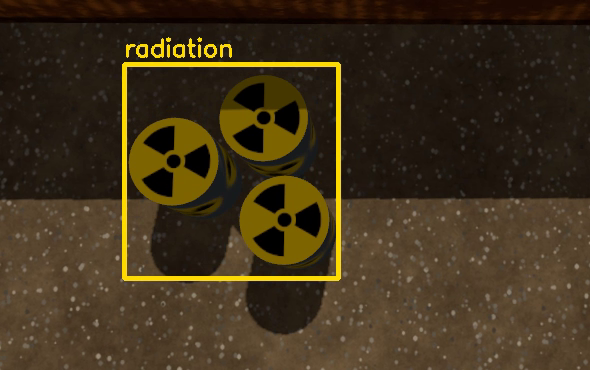
\includegraphics[width=\columnwidth]{camera.png}
\caption{Crop of the UAV image with radiation signs detected on barrel lids. Boxes and labels are published by the sign detector during the mission.}
\label{fig:camera}
\end{figure}

The detector converts the sign's image position to a map position using the camera's field of view and the UAV's position and orientation. It assumes that signs lie on a horizontal barrel-lid plane at \SI{0.9}{\metre}. The detector uses the buffered pose closest to the image timestamp. Three sightings are required before publication; same-type sightings within \SI{1.5}{\metre} are averaged into one sign record. Projection errors can still split one physical sign into several records or merge nearby signs. Pose timing, perspective and the assumed plane height affect the estimated position.

At a sign target, the UAV first reaches a \SI{0.4}{\metre} tolerance in horizontal position and altitude. It then averages at least five fresh readings received after arrival. The alarm thresholds are \SI{8}{\ppm} for gas and \SI{0.4}{\micro\sievert\per\hour} for radiation. Targets outside the flight area are clipped to its boundary. A sign does not directly create a candidate: the average must reach the corresponding alarm threshold.

Without a sign, an alarm starts a compass search with \SI{2}{\metre} steps. It measures the centre and four axis-aligned neighbours, then examines the neighbours of the best point once more if the value improves. There are at most nine probes, each averaging at least five fresh readings after arrival. Travelling between probes and collecting new readings account for the time spent over an elevated area. Each inspection has a \SI{25}{\second} limit, including movement. A newly published sign of the same type can redirect the search into a new direct inspection. The highest measured point becomes a candidate if it reaches the alarm threshold. A new candidate is suppressed if it lies within \SI{6}{\metre} of an existing candidate of the same type. Previous search origins are also remembered to limit repeated inspections.

These rules locate a measured hazardous area. A short search or a label beside a leak may leave the reported point away from the source itself. This distance rule can merge nearby sources of the same type, and observations farther apart can still refer to the same source.

\subsection{Ground allocation, navigation and confirmation}
The coordinator chooses the eligible UGV with the shortest straight-line distance to the candidate. An eligible robot must be idle, have a reported position and a ready Nav2 server, and must not have already failed this candidate. Previous completed work does not affect the choice. Tasks wait in arrival order when no robot is available. The distance comparison ignores obstacles, so the selected robot may have a longer actual route than the other robot.

Each UGV has differential drive and a \SI{10}{\hertz}, 360-beam planar laser scanner. Separate Nav2 instances use AMCL, the NavFn planner, the DWB local controller and two-dimensional obstacle and inflation layers. Maximum forward speed is \SI{0.26}{\metre\per\second}. AMCL uses 180 laser beams and updates after \SI{0.05}{\metre} or \SI{0.05}{\radian} of movement. The static map supports localisation; live laser observations update navigation costmaps. Optional UGV front cameras and a fixed overview camera record the demonstration only. They are disabled by default and do not supply mission decisions.

The coordinator searches nearby map cells in successive square rings, up to \SI{3}{\metre} along each map axis, and requires \SI{0.5}{\metre} obstacle clearance. This allows measurement beside a container instead of requesting an occupied cell. Nav2 must report success, and the reported robot position must lie within \SI{0.75}{\metre} of the assigned goal. The coordinator then collects finite, fresh readings for \SI{3}{\second}, requiring at least three samples. A mean of at least \SI{5}{\ppm} or \SI{0.5}{\micro\sievert\per\hour} confirms the corresponding hazard. These are demonstration settings, not exposure limits.

A completed measurement below threshold publishes an unconfirmed result. Navigation failure or missing samples does not count as a negative measurement: the task is offered to the other UGV. After both robots fail, it remains unconfirmed. This bounds reassignment without treating unsuccessful navigation as evidence about the field.

\subsection{Mission visualisation}
RViz displays the occupancy map, signs, candidates, ground checks, robot positions and navigation paths. Ground measurements colour visited cells blue, yellow or red according to their values. Fig.~\ref{fig:map} shows an equivalent live view rendered from the same ROS topics for the demonstration video. Unvisited cells remain unassessed, and airborne readings do not classify ground cells. Each \SI{1}{\metre} cell retains the highest recorded severity level. Blue indicates a low reading, yellow an elevated reading and red a high reading. Gas thresholds are 5 and \SI{20}{\ppm}; radiation thresholds are 0.5 and \SI{2}{\micro\sievert\per\hour}. These colours summarise sampled ground locations and do not certify site safety.

\begin{figure}[t]
\centering
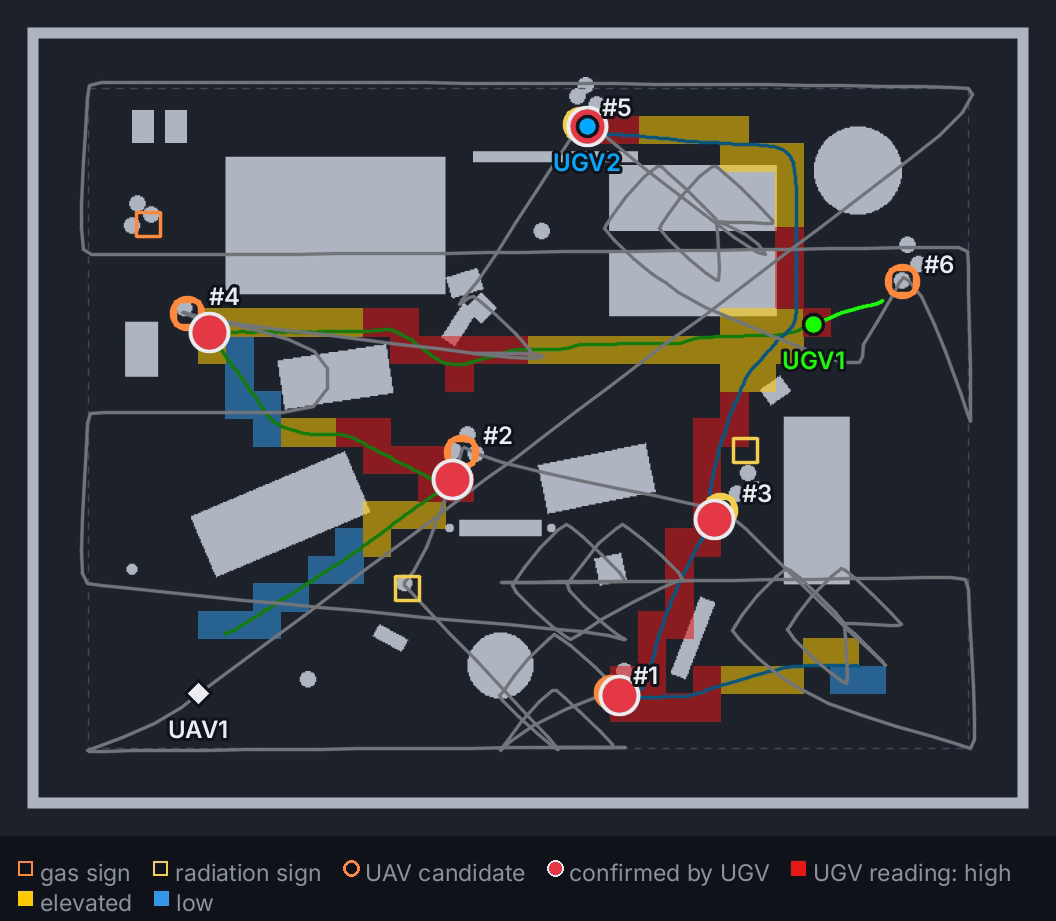
\includegraphics[width=\columnwidth]{hazard_map.png}
\caption{Live hazard map from ROS topics during the recorded mission with six active sources. Pale cells are obstacles; coloured cells record UGV measurements. Rings mark aerial candidates, and filled red circles mark positive ground checks. Reference source positions are not displayed.}
\label{fig:map}
\end{figure}

\section{Experiments and results}
\subsection{Setup and metrics}
The evaluation logger records candidates and ground checks in a comma-separated values (CSV) file. Position error is the straight-line distance, in metres, between the reported position and the nearest reference source of the same type. A gas observation is compared with gas sources, and a radiation observation with radiation sources. This measures location accuracy, not the accuracy of the gas or radiation value. Multiple observations can refer to the same source, so distinct reference sources are counted separately from detection events.

Three completed headless Gazebo trials (R1, R2 and R3) use the same six-source site, robot start positions and controller settings. UGVs start at (-11, -7.8) and (12, -9) metres; the UAV starts at (-12, -10) metres. Each trial restarts the simulation. Sensor noise is sampled without a fixed common random seed. The figures show a separate recording of this configuration. A radiation-labelled barrel at (-4.5, -6.0) metres provides the unsupported visual cue.

\begin{table}[t]
\caption{Results of three trials in the six-source scenario}
\label{tab:runs}
\centering
\small
\begin{tabular}{@{}ccrrr@{}}
\toprule
Run & \shortstack{Sources\\confirmed} & \shortstack{Last check\\(s)} & \shortstack{Mean UAV\\error (m)} & \shortstack{Mean UGV\\error (m)}\\
\midrule
R1 & 6/6 & 294.1 & 1.48 & 1.67\\
R2 & 6/6 & 280.3 & 1.51 & 1.68\\
R3 & 6/6 & 292.3 & 1.50 & 1.71\\
\bottomrule
\end{tabular}
\end{table}

Table~\ref{tab:runs} reports the elapsed simulation time from when the logger starts timing to the final positive ground check. Simulator startup is excluded. Mean UAV error averages the position errors of the aerial candidates; mean UGV error averages those of the positive ground checks. The UAV landed before the final ground confirmation in all three trials. This timing includes ground work completed after landing.

\subsection{Measured results}
Each trial produced six aerial candidates and six positive ground checks. Nearest-source matching associated these checks with six distinct source names, as reported in Table~\ref{tab:runs}. Each UGV completed three checks. This distribution follows availability and distance; there is no work-history penalty or task-count balancing. The UAV's stopping condition remains route completion regardless of the candidate count.

\begin{table}[t]
\caption{Source-level results for trial R1}
\label{tab:sources}
\centering
\small
\begin{tabular}{@{}lrrrr@{}}
\toprule
Source & \shortstack{UAV error\\(m)} & \shortstack{UGV error\\(m)} & \shortstack{Ground\\reading} & \shortstack{Check\\(s)}\\
\midrule
Gas 4 & 0.87 & 0.92 & 38.297 & 79.1\\
Gas 1 & 2.04 & 2.83 & 25.982 & 91.1\\
Radiation 1 & 0.44 & 0.32 & 17.386 & 116.1\\
Gas 3 & 3.55 & 4.58 & 8.265 & 186.1\\
Radiation 2 & 0.75 & 1.12 & 8.587 & 248.1\\
Gas 2 & 1.21 & 0.22 & 40.773 & 294.1\\
\bottomrule
\end{tabular}
\par\smallskip
\footnotesize Radiation values are in \si{\micro\sievert\per\hour}; gas values are in ppm.
\end{table}

Table~\ref{tab:sources} illustrates the distinction between confirmation and source localisation. For Gas 3, a sign near the edge of the elevated field requested an inspection before the UAV reached the source's closest labels. The UGV then measured at an accessible location. Its reading exceeded the confirmation threshold, although position error increased from \SI{3.55}{\metre} to \SI{4.58}{\metre}. Gas 1 shows the same effect at a smaller scale. Ground confirmation establishes an elevated local reading and does not necessarily improve the estimated source position.

The source without a matching sign and the sign without a source test the role of the camera. In all three runs, the UAV inspected the radiation-labelled barrel without a source, measured an average below the alarm threshold and published no candidate. Gas 4 has no matching gas warning sign nearby. In each run, a gas alarm on the first survey lane started a local search; its candidate lay 0.87 to \SI{0.90}{\metre} from the source, and \texttt{ugv2} confirmed it. These trials show both paths to inspection: the camera can request a check, and sensor readings can detect a hazard without a matching sign.

\subsection{Validation and limitations}
Candidate identifiers count observations, not physical sources. Spatial grouping reduces repeated reports but cannot guarantee one candidate per source. An additional recording attempt generated seven candidates for the same six-source configuration, with two associated with Radiation 1. It ended while the Radiation 2 ground check was pending, so it is excluded from the completed trials in Table~\ref{tab:runs}. This case also shows why a count of positive checks alone is insufficient to judge mission completion.

The three ROS packages build successfully, and all 42 automated tests pass. These tests cover field calculations, search bounds, visual detection and projection, allocation and confirmation conditions, and separation between actual sensor position and reported navigation position. The Gazebo runs exercise the interaction between these components. They do not replace evaluation across different layouts, field conditions or physical robots.

\section{Conclusion}
\subsection{Discussion of results}
The project implements a cooperative application through aerial survey, shared candidates and ground confirmation. It combines a custom industrial scenario and mission nodes with existing simulation models and Nav2. The UAV makes decisions from camera detections, measured values and navigation poses without reading the hidden field model. The UGV coordinator uses the nearest available robot and a bounded retry policy.

The three completed trials support operation in the tested six-source scenario. All reference sources received positive ground checks, including Gas 4 without a matching gas sign. The unsupported radiation sign produced no candidate in these trials. Ground confirmation checks an elevated local measurement and does not perform a second search for the source. Repeated trials in one fixed layout do not establish reliability under arbitrary source placements or show that this policy is faster than alternative search or allocation methods.

\subsection{Limitations and future work}
The main limitations are ideal UAV localisation, static synthetic fields, fixed visual colour rules and a known sign-height plane. The method also assumes a prepared obstacle map and known initial robot poses. Fixed survey spacing can miss weak sources, while spatial grouping can merge nearby sources or allow repeated reports of one field. Straight-line allocation ignores route length, and accessible goals can be offset from the source. Further evaluation should vary source positions and strengths and include more unsupported signs and unlabelled leaks. More realistic sensing and uncertain UAV localisation should precede physical deployment. If assignment efficiency becomes a measured bottleneck, planned route cost can replace Euclidean distance without introducing a work-history penalty.

\bibliographystyle{IEEEtran}
\bibliography{references}
\end{document}
